\subsection{More Examples} 

(Answers to M\Alph{subsection} problems are on page \pageref{examples_prob_answers}.)



\begin{Exercise}
The graph below shows the number of decays of the excited state \isotope[137\mathrm{m}][56]{Ba} measured as a function of time, just as you did in Lab~\ref{nuclear_decay_lab}. (a)~Estimate by eye the half-life $t_{1/2}$ of the excited state of \isotope[137{\rm m}]{Ba} from the graph below. (I don't want you actually calculate anything.  I want you to think about what ``half-life'' means and give me a rough value for it.)  (b)~Estimate by eye the ``mean lifetime'' $\tau$ from the graph below.  (c)~Based on your previous answer, estimate the value of the decay constant $\lambda$, including the correct units. (Bear in mind that this $\lambda$ has nothing to do with any wavelength, other than that they happen to use the same Greek letter.) 
\begin{center}
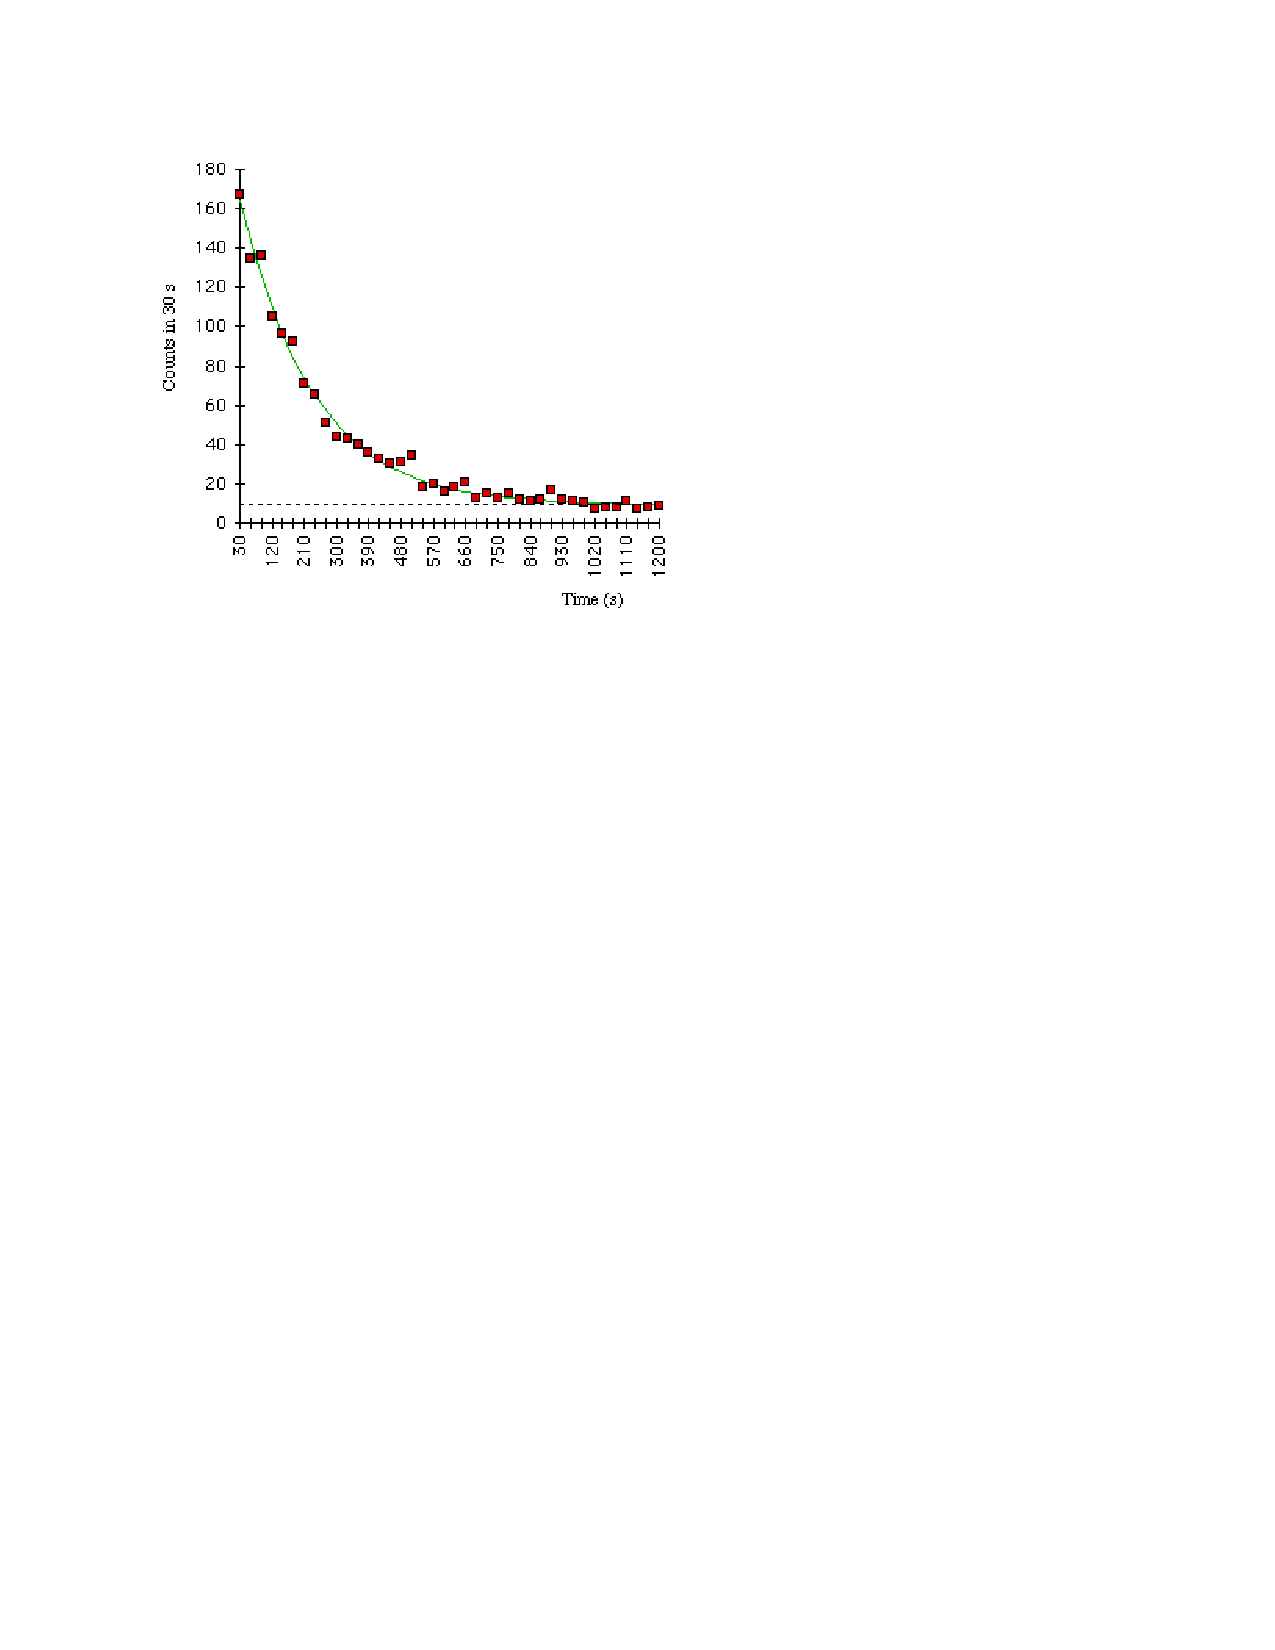
\includegraphics{M_problems/lorentz/barium_decay_graph.pdf}
\index{color page}
\end{center}
 \end{Exercise}
\begin{Answer}
(a) About 210 seconds (b) About 300 seconds (c) $\approx 3.3 \times 10^{-3}~{\rm s}^{-1}$
\end{Answer}

\begin{Exercise}
The radioactive isotope \isotope[15]{C} has a half-life of 2.449~seconds.  (a)~Calculate the mean lifetime $\tau$ and decay constant $\lambda$ for \isotope[15]{C}.  (b)~Suppose you begin at time $t=0$ with a sample of $N_0=10,000$ atoms of \isotope[15]{C}.  How many atoms $N$ do you expect to be left at time $t=8$ seconds?  (c)~What percent of the original atoms (that is, $N/N_0$, expressed as a percentage) would you expect to remain at time $t=11$~seconds?
\end{Exercise}
\begin{Answer}
(a) $\tau=3.53$~s, $\lambda=0.283~{\rm s}^{-1}$  (b)~About 1039 atoms, though due to statistical fluctuations it might be a little higher or lower, in the same way that if you flipped 10,000 coins, you might end up with results slightly different from 5000 heads and 5000 tails.  (c)~4.4\%
\end{Answer}


\begin{Exercise}
At rest, neutrons that are not bound within atomic nuclei have a mean lifetime of $\tau=14.692$~minutes.  The fusion of deuterium and tritium nuclei (\isotope[2]{H} and \isotope[3]{H}, respectively), in a laboratory or in the sun, produces helium (\isotope[4]{He}) and a very high-energy neutron that travels at 17.3\% of the speed of light.  What is the mean lifetime of these fast neutrons, in seconds, in the ``laboratory'' reference frame (that is, the reference frame of the Earth)?  You'll need to keep five significant digits in your answer, to make it clear that your answer is different from the 
14.692~minutes in the reference frame of the neutron.
\end{Exercise}
\begin{Answer}
894.99 seconds.
\end{Answer}

\begin{Exercise}[difficulty=0]
Anna has recently taken up pole vaulting, and owns a 10~m long pole (its proper length).  Bob has taken up farming, and owns an 8~m long barn (also its proper length) with a door on each end.  Anna runs very fast towards the open barn; in fact, she runs so fast that in the reference frame of Bob and the barn, the pole's length is Lorentz contracted to just 6~meters.  When Bob sees that Anna is exactly centered inside the barn, he pushes a button that closes both doors very quickly.  
\begin{itemize}
\item Bob says, ``Hah! I've closed Anna and her pole inside my barn!''  
\item But in Anna's reference frame, it is the barn that is Lorentz contracted.  Anna says, ``My pole is 10 meters long, and your dinky little barn is clearly less than 8 meters long.  Since your barn is shorter than my pole, you couldn't possibly close me and my pole inside of it!''
\end{itemize}
\begin{center}
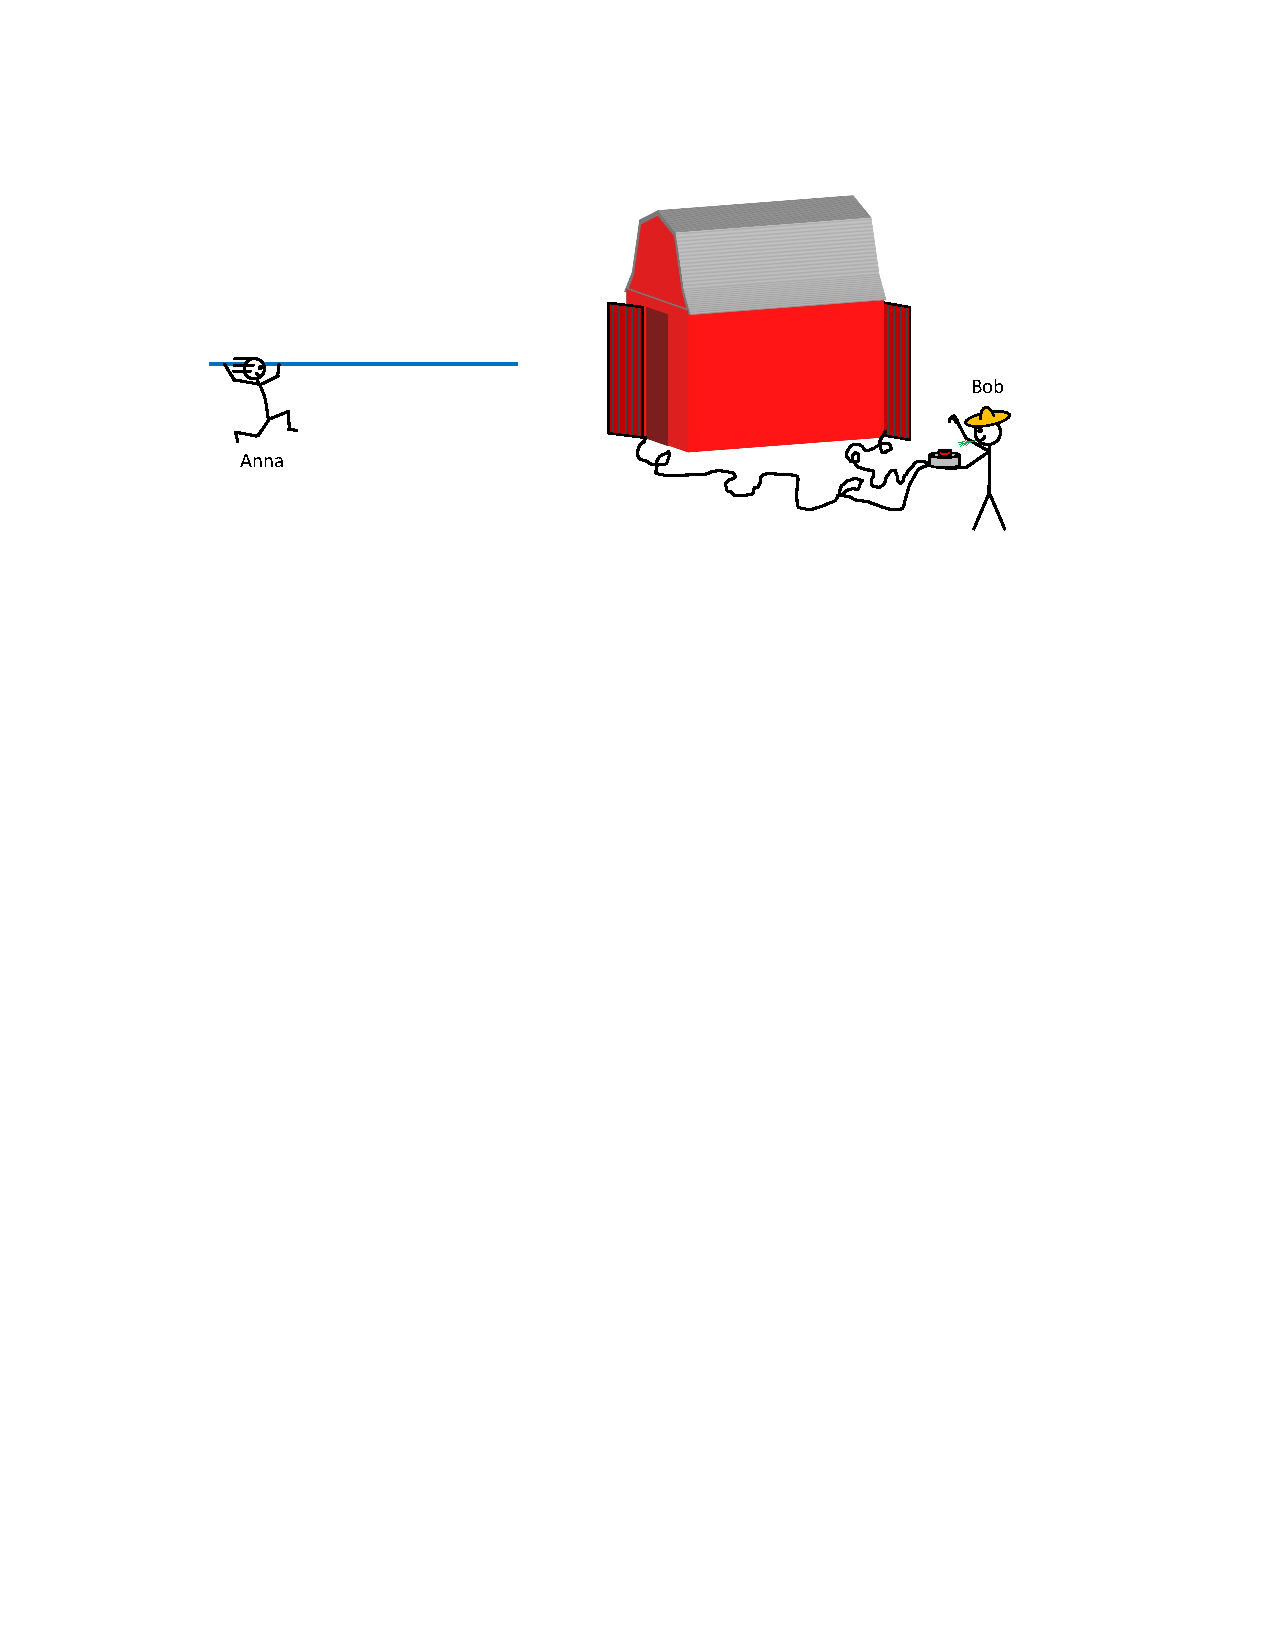
\includegraphics[scale=0.85]{M_problems/velocities_causality/pole_and_barn_color.pdf}
\index{color page}
\end{center}
Who is correct?  Anna, or Bob?  (Remarks: this problem is actually quite tricky, and we'll address it in our next class.  Take five or ten minutes to think about it and write down your thoughts, but don't spend more time on it than that.)
\end{Exercise}



\begin{Exercise}[difficulty=0]
Bob and Anna are the same age.  While Bob stays on Earth, Anna sets off at a constant speed $v=0.8c$ ($\gamma=1.67$) to visit another planet.  In the Earth reference frame, the planet is 24~ly away.  Once there, she turns around and comes back, also at $v=0.8c$.  (a) According to Bob, how long is Anna gone?  (b) According to Anna, how long is she gone?  (c) Suppose that instead of staying on Earth, Bob is floating in a spaceship (engines off) just outside our solar system during Anna's journey.  Does this affect your answers to parts (a) and (b)?  (d) Suppose that instead of traveling to a specific planet, Anna simply travels away in a random direction to a distance 24 ly away from Bob (according to Bob).  Does that change your answers to parts (a) and (b)?  (e) Just before they reunite, Anna radios Bob, saying ``Hey, from my spaceship, it looks like you had a velocity of $0.8c$ away from me, and then you turned around and had a velocity of $0.8c$ towards me.  I expect that when I see you again, you will not have aged as much, and will look much younger than me.''  Bob expects Anna to be younger.  But Anna also expects Bob to be younger.  Can they both be right?  Explain how to resolve this apparent paradox.
\end{Exercise}
\begin{Answer}
(a) 60 years (b) 36 years
\end{Answer}





\bigskip\bigskip\bigskip
\pagebreak[3]
\textbf{Answers to Selected {\thesubsection} Problems:}
\label{examples_prob_answers}
%\shipoutExercise
\shipoutAnswer

\cleardoublepage